
% Default to the notebook output style

    


% Inherit from the specified cell style.




    
\documentclass[11pt]{article}

    
    
    \usepackage[T1]{fontenc}
    % Nicer default font than Computer Modern for most use cases
    \usepackage{palatino}

    % Basic figure setup, for now with no caption control since it's done
    % automatically by Pandoc (which extracts ![](path) syntax from Markdown).
    \usepackage{graphicx}
    % We will generate all images so they have a width \maxwidth. This means
    % that they will get their normal width if they fit onto the page, but
    % are scaled down if they would overflow the margins.
    \makeatletter
    \def\maxwidth{\ifdim\Gin@nat@width>\linewidth\linewidth
    \else\Gin@nat@width\fi}
    \makeatother
    \let\Oldincludegraphics\includegraphics
    % Set max figure width to be 80% of text width, for now hardcoded.
    \renewcommand{\includegraphics}[1]{\Oldincludegraphics[width=.8\maxwidth]{#1}}
    % Ensure that by default, figures have no caption (until we provide a
    % proper Figure object with a Caption API and a way to capture that
    % in the conversion process - todo).
    \usepackage{caption}
    \DeclareCaptionLabelFormat{nolabel}{}
    \captionsetup{labelformat=nolabel}

    \usepackage{adjustbox} % Used to constrain images to a maximum size 
    \usepackage{xcolor} % Allow colors to be defined
    \usepackage{enumerate} % Needed for markdown enumerations to work
    \usepackage{geometry} % Used to adjust the document margins
    \usepackage{amsmath} % Equations
    \usepackage{amssymb} % Equations
    \usepackage{textcomp} % defines textquotesingle
    % Hack from http://tex.stackexchange.com/a/47451/13684:
    \AtBeginDocument{%
        \def\PYZsq{\textquotesingle}% Upright quotes in Pygmentized code
    }
    \usepackage{upquote} % Upright quotes for verbatim code
    \usepackage{eurosym} % defines \euro
    \usepackage[mathletters]{ucs} % Extended unicode (utf-8) support
    \usepackage[utf8x]{inputenc} % Allow utf-8 characters in the tex document
    \usepackage{fancyvrb} % verbatim replacement that allows latex
    \usepackage{grffile} % extends the file name processing of package graphics 
                         % to support a larger range 
    % The hyperref package gives us a pdf with properly built
    % internal navigation ('pdf bookmarks' for the table of contents,
    % internal cross-reference links, web links for URLs, etc.)
    \usepackage{hyperref}
    \usepackage{longtable} % longtable support required by pandoc >1.10
    \usepackage{booktabs}  % table support for pandoc > 1.12.2
    \usepackage[normalem]{ulem} % ulem is needed to support strikethroughs (\sout)
                                % normalem makes italics be italics, not underlines
    

    
    
    % Colors for the hyperref package
    \definecolor{urlcolor}{rgb}{0,.145,.698}
    \definecolor{linkcolor}{rgb}{.71,0.21,0.01}
    \definecolor{citecolor}{rgb}{.12,.54,.11}

    % ANSI colors
    \definecolor{ansi-black}{HTML}{3E424D}
    \definecolor{ansi-black-intense}{HTML}{282C36}
    \definecolor{ansi-red}{HTML}{E75C58}
    \definecolor{ansi-red-intense}{HTML}{B22B31}
    \definecolor{ansi-green}{HTML}{00A250}
    \definecolor{ansi-green-intense}{HTML}{007427}
    \definecolor{ansi-yellow}{HTML}{DDB62B}
    \definecolor{ansi-yellow-intense}{HTML}{B27D12}
    \definecolor{ansi-blue}{HTML}{208FFB}
    \definecolor{ansi-blue-intense}{HTML}{0065CA}
    \definecolor{ansi-magenta}{HTML}{D160C4}
    \definecolor{ansi-magenta-intense}{HTML}{A03196}
    \definecolor{ansi-cyan}{HTML}{60C6C8}
    \definecolor{ansi-cyan-intense}{HTML}{258F8F}
    \definecolor{ansi-white}{HTML}{C5C1B4}
    \definecolor{ansi-white-intense}{HTML}{A1A6B2}

    % commands and environments needed by pandoc snippets
    % extracted from the output of `pandoc -s`
    \providecommand{\tightlist}{%
      \setlength{\itemsep}{0pt}\setlength{\parskip}{0pt}}
    \DefineVerbatimEnvironment{Highlighting}{Verbatim}{commandchars=\\\{\}}
    % Add ',fontsize=\small' for more characters per line
    \newenvironment{Shaded}{}{}
    \newcommand{\KeywordTok}[1]{\textcolor[rgb]{0.00,0.44,0.13}{\textbf{{#1}}}}
    \newcommand{\DataTypeTok}[1]{\textcolor[rgb]{0.56,0.13,0.00}{{#1}}}
    \newcommand{\DecValTok}[1]{\textcolor[rgb]{0.25,0.63,0.44}{{#1}}}
    \newcommand{\BaseNTok}[1]{\textcolor[rgb]{0.25,0.63,0.44}{{#1}}}
    \newcommand{\FloatTok}[1]{\textcolor[rgb]{0.25,0.63,0.44}{{#1}}}
    \newcommand{\CharTok}[1]{\textcolor[rgb]{0.25,0.44,0.63}{{#1}}}
    \newcommand{\StringTok}[1]{\textcolor[rgb]{0.25,0.44,0.63}{{#1}}}
    \newcommand{\CommentTok}[1]{\textcolor[rgb]{0.38,0.63,0.69}{\textit{{#1}}}}
    \newcommand{\OtherTok}[1]{\textcolor[rgb]{0.00,0.44,0.13}{{#1}}}
    \newcommand{\AlertTok}[1]{\textcolor[rgb]{1.00,0.00,0.00}{\textbf{{#1}}}}
    \newcommand{\FunctionTok}[1]{\textcolor[rgb]{0.02,0.16,0.49}{{#1}}}
    \newcommand{\RegionMarkerTok}[1]{{#1}}
    \newcommand{\ErrorTok}[1]{\textcolor[rgb]{1.00,0.00,0.00}{\textbf{{#1}}}}
    \newcommand{\NormalTok}[1]{{#1}}
    
    % Additional commands for more recent versions of Pandoc
    \newcommand{\ConstantTok}[1]{\textcolor[rgb]{0.53,0.00,0.00}{{#1}}}
    \newcommand{\SpecialCharTok}[1]{\textcolor[rgb]{0.25,0.44,0.63}{{#1}}}
    \newcommand{\VerbatimStringTok}[1]{\textcolor[rgb]{0.25,0.44,0.63}{{#1}}}
    \newcommand{\SpecialStringTok}[1]{\textcolor[rgb]{0.73,0.40,0.53}{{#1}}}
    \newcommand{\ImportTok}[1]{{#1}}
    \newcommand{\DocumentationTok}[1]{\textcolor[rgb]{0.73,0.13,0.13}{\textit{{#1}}}}
    \newcommand{\AnnotationTok}[1]{\textcolor[rgb]{0.38,0.63,0.69}{\textbf{\textit{{#1}}}}}
    \newcommand{\CommentVarTok}[1]{\textcolor[rgb]{0.38,0.63,0.69}{\textbf{\textit{{#1}}}}}
    \newcommand{\VariableTok}[1]{\textcolor[rgb]{0.10,0.09,0.49}{{#1}}}
    \newcommand{\ControlFlowTok}[1]{\textcolor[rgb]{0.00,0.44,0.13}{\textbf{{#1}}}}
    \newcommand{\OperatorTok}[1]{\textcolor[rgb]{0.40,0.40,0.40}{{#1}}}
    \newcommand{\BuiltInTok}[1]{{#1}}
    \newcommand{\ExtensionTok}[1]{{#1}}
    \newcommand{\PreprocessorTok}[1]{\textcolor[rgb]{0.74,0.48,0.00}{{#1}}}
    \newcommand{\AttributeTok}[1]{\textcolor[rgb]{0.49,0.56,0.16}{{#1}}}
    \newcommand{\InformationTok}[1]{\textcolor[rgb]{0.38,0.63,0.69}{\textbf{\textit{{#1}}}}}
    \newcommand{\WarningTok}[1]{\textcolor[rgb]{0.38,0.63,0.69}{\textbf{\textit{{#1}}}}}
    
    
    % Define a nice break command that doesn't care if a line doesn't already
    % exist.
    \def\br{\hspace*{\fill} \\* }
    % Math Jax compatability definitions
    \def\gt{>}
    \def\lt{<}
    % Document parameters
    \title{latex\_env\_doc}
    
    
    

    % Pygments definitions
    
\makeatletter
\def\PY@reset{\let\PY@it=\relax \let\PY@bf=\relax%
    \let\PY@ul=\relax \let\PY@tc=\relax%
    \let\PY@bc=\relax \let\PY@ff=\relax}
\def\PY@tok#1{\csname PY@tok@#1\endcsname}
\def\PY@toks#1+{\ifx\relax#1\empty\else%
    \PY@tok{#1}\expandafter\PY@toks\fi}
\def\PY@do#1{\PY@bc{\PY@tc{\PY@ul{%
    \PY@it{\PY@bf{\PY@ff{#1}}}}}}}
\def\PY#1#2{\PY@reset\PY@toks#1+\relax+\PY@do{#2}}

\expandafter\def\csname PY@tok@kp\endcsname{\def\PY@tc##1{\textcolor[rgb]{0.00,0.50,0.00}{##1}}}
\expandafter\def\csname PY@tok@err\endcsname{\def\PY@bc##1{\setlength{\fboxsep}{0pt}\fcolorbox[rgb]{1.00,0.00,0.00}{1,1,1}{\strut ##1}}}
\expandafter\def\csname PY@tok@nn\endcsname{\let\PY@bf=\textbf\def\PY@tc##1{\textcolor[rgb]{0.00,0.00,1.00}{##1}}}
\expandafter\def\csname PY@tok@gd\endcsname{\def\PY@tc##1{\textcolor[rgb]{0.63,0.00,0.00}{##1}}}
\expandafter\def\csname PY@tok@gh\endcsname{\let\PY@bf=\textbf\def\PY@tc##1{\textcolor[rgb]{0.00,0.00,0.50}{##1}}}
\expandafter\def\csname PY@tok@kr\endcsname{\let\PY@bf=\textbf\def\PY@tc##1{\textcolor[rgb]{0.00,0.50,0.00}{##1}}}
\expandafter\def\csname PY@tok@vc\endcsname{\def\PY@tc##1{\textcolor[rgb]{0.10,0.09,0.49}{##1}}}
\expandafter\def\csname PY@tok@nd\endcsname{\def\PY@tc##1{\textcolor[rgb]{0.67,0.13,1.00}{##1}}}
\expandafter\def\csname PY@tok@cs\endcsname{\let\PY@it=\textit\def\PY@tc##1{\textcolor[rgb]{0.25,0.50,0.50}{##1}}}
\expandafter\def\csname PY@tok@se\endcsname{\let\PY@bf=\textbf\def\PY@tc##1{\textcolor[rgb]{0.73,0.40,0.13}{##1}}}
\expandafter\def\csname PY@tok@ow\endcsname{\let\PY@bf=\textbf\def\PY@tc##1{\textcolor[rgb]{0.67,0.13,1.00}{##1}}}
\expandafter\def\csname PY@tok@mo\endcsname{\def\PY@tc##1{\textcolor[rgb]{0.40,0.40,0.40}{##1}}}
\expandafter\def\csname PY@tok@kd\endcsname{\let\PY@bf=\textbf\def\PY@tc##1{\textcolor[rgb]{0.00,0.50,0.00}{##1}}}
\expandafter\def\csname PY@tok@gs\endcsname{\let\PY@bf=\textbf}
\expandafter\def\csname PY@tok@kc\endcsname{\let\PY@bf=\textbf\def\PY@tc##1{\textcolor[rgb]{0.00,0.50,0.00}{##1}}}
\expandafter\def\csname PY@tok@go\endcsname{\def\PY@tc##1{\textcolor[rgb]{0.53,0.53,0.53}{##1}}}
\expandafter\def\csname PY@tok@s\endcsname{\def\PY@tc##1{\textcolor[rgb]{0.73,0.13,0.13}{##1}}}
\expandafter\def\csname PY@tok@kn\endcsname{\let\PY@bf=\textbf\def\PY@tc##1{\textcolor[rgb]{0.00,0.50,0.00}{##1}}}
\expandafter\def\csname PY@tok@c\endcsname{\let\PY@it=\textit\def\PY@tc##1{\textcolor[rgb]{0.25,0.50,0.50}{##1}}}
\expandafter\def\csname PY@tok@no\endcsname{\def\PY@tc##1{\textcolor[rgb]{0.53,0.00,0.00}{##1}}}
\expandafter\def\csname PY@tok@gi\endcsname{\def\PY@tc##1{\textcolor[rgb]{0.00,0.63,0.00}{##1}}}
\expandafter\def\csname PY@tok@nv\endcsname{\def\PY@tc##1{\textcolor[rgb]{0.10,0.09,0.49}{##1}}}
\expandafter\def\csname PY@tok@sb\endcsname{\def\PY@tc##1{\textcolor[rgb]{0.73,0.13,0.13}{##1}}}
\expandafter\def\csname PY@tok@il\endcsname{\def\PY@tc##1{\textcolor[rgb]{0.40,0.40,0.40}{##1}}}
\expandafter\def\csname PY@tok@gt\endcsname{\def\PY@tc##1{\textcolor[rgb]{0.00,0.27,0.87}{##1}}}
\expandafter\def\csname PY@tok@vg\endcsname{\def\PY@tc##1{\textcolor[rgb]{0.10,0.09,0.49}{##1}}}
\expandafter\def\csname PY@tok@kt\endcsname{\def\PY@tc##1{\textcolor[rgb]{0.69,0.00,0.25}{##1}}}
\expandafter\def\csname PY@tok@sh\endcsname{\def\PY@tc##1{\textcolor[rgb]{0.73,0.13,0.13}{##1}}}
\expandafter\def\csname PY@tok@nl\endcsname{\def\PY@tc##1{\textcolor[rgb]{0.63,0.63,0.00}{##1}}}
\expandafter\def\csname PY@tok@ch\endcsname{\let\PY@it=\textit\def\PY@tc##1{\textcolor[rgb]{0.25,0.50,0.50}{##1}}}
\expandafter\def\csname PY@tok@bp\endcsname{\def\PY@tc##1{\textcolor[rgb]{0.00,0.50,0.00}{##1}}}
\expandafter\def\csname PY@tok@na\endcsname{\def\PY@tc##1{\textcolor[rgb]{0.49,0.56,0.16}{##1}}}
\expandafter\def\csname PY@tok@nf\endcsname{\def\PY@tc##1{\textcolor[rgb]{0.00,0.00,1.00}{##1}}}
\expandafter\def\csname PY@tok@m\endcsname{\def\PY@tc##1{\textcolor[rgb]{0.40,0.40,0.40}{##1}}}
\expandafter\def\csname PY@tok@vi\endcsname{\def\PY@tc##1{\textcolor[rgb]{0.10,0.09,0.49}{##1}}}
\expandafter\def\csname PY@tok@gr\endcsname{\def\PY@tc##1{\textcolor[rgb]{1.00,0.00,0.00}{##1}}}
\expandafter\def\csname PY@tok@ge\endcsname{\let\PY@it=\textit}
\expandafter\def\csname PY@tok@ni\endcsname{\let\PY@bf=\textbf\def\PY@tc##1{\textcolor[rgb]{0.60,0.60,0.60}{##1}}}
\expandafter\def\csname PY@tok@cp\endcsname{\def\PY@tc##1{\textcolor[rgb]{0.74,0.48,0.00}{##1}}}
\expandafter\def\csname PY@tok@sx\endcsname{\def\PY@tc##1{\textcolor[rgb]{0.00,0.50,0.00}{##1}}}
\expandafter\def\csname PY@tok@mf\endcsname{\def\PY@tc##1{\textcolor[rgb]{0.40,0.40,0.40}{##1}}}
\expandafter\def\csname PY@tok@nb\endcsname{\def\PY@tc##1{\textcolor[rgb]{0.00,0.50,0.00}{##1}}}
\expandafter\def\csname PY@tok@gu\endcsname{\let\PY@bf=\textbf\def\PY@tc##1{\textcolor[rgb]{0.50,0.00,0.50}{##1}}}
\expandafter\def\csname PY@tok@si\endcsname{\let\PY@bf=\textbf\def\PY@tc##1{\textcolor[rgb]{0.73,0.40,0.53}{##1}}}
\expandafter\def\csname PY@tok@cpf\endcsname{\let\PY@it=\textit\def\PY@tc##1{\textcolor[rgb]{0.25,0.50,0.50}{##1}}}
\expandafter\def\csname PY@tok@sr\endcsname{\def\PY@tc##1{\textcolor[rgb]{0.73,0.40,0.53}{##1}}}
\expandafter\def\csname PY@tok@gp\endcsname{\let\PY@bf=\textbf\def\PY@tc##1{\textcolor[rgb]{0.00,0.00,0.50}{##1}}}
\expandafter\def\csname PY@tok@mb\endcsname{\def\PY@tc##1{\textcolor[rgb]{0.40,0.40,0.40}{##1}}}
\expandafter\def\csname PY@tok@cm\endcsname{\let\PY@it=\textit\def\PY@tc##1{\textcolor[rgb]{0.25,0.50,0.50}{##1}}}
\expandafter\def\csname PY@tok@w\endcsname{\def\PY@tc##1{\textcolor[rgb]{0.73,0.73,0.73}{##1}}}
\expandafter\def\csname PY@tok@s2\endcsname{\def\PY@tc##1{\textcolor[rgb]{0.73,0.13,0.13}{##1}}}
\expandafter\def\csname PY@tok@sc\endcsname{\def\PY@tc##1{\textcolor[rgb]{0.73,0.13,0.13}{##1}}}
\expandafter\def\csname PY@tok@o\endcsname{\def\PY@tc##1{\textcolor[rgb]{0.40,0.40,0.40}{##1}}}
\expandafter\def\csname PY@tok@nc\endcsname{\let\PY@bf=\textbf\def\PY@tc##1{\textcolor[rgb]{0.00,0.00,1.00}{##1}}}
\expandafter\def\csname PY@tok@ss\endcsname{\def\PY@tc##1{\textcolor[rgb]{0.10,0.09,0.49}{##1}}}
\expandafter\def\csname PY@tok@mh\endcsname{\def\PY@tc##1{\textcolor[rgb]{0.40,0.40,0.40}{##1}}}
\expandafter\def\csname PY@tok@sd\endcsname{\let\PY@it=\textit\def\PY@tc##1{\textcolor[rgb]{0.73,0.13,0.13}{##1}}}
\expandafter\def\csname PY@tok@k\endcsname{\let\PY@bf=\textbf\def\PY@tc##1{\textcolor[rgb]{0.00,0.50,0.00}{##1}}}
\expandafter\def\csname PY@tok@c1\endcsname{\let\PY@it=\textit\def\PY@tc##1{\textcolor[rgb]{0.25,0.50,0.50}{##1}}}
\expandafter\def\csname PY@tok@nt\endcsname{\let\PY@bf=\textbf\def\PY@tc##1{\textcolor[rgb]{0.00,0.50,0.00}{##1}}}
\expandafter\def\csname PY@tok@ne\endcsname{\let\PY@bf=\textbf\def\PY@tc##1{\textcolor[rgb]{0.82,0.25,0.23}{##1}}}
\expandafter\def\csname PY@tok@mi\endcsname{\def\PY@tc##1{\textcolor[rgb]{0.40,0.40,0.40}{##1}}}
\expandafter\def\csname PY@tok@s1\endcsname{\def\PY@tc##1{\textcolor[rgb]{0.73,0.13,0.13}{##1}}}

\def\PYZbs{\char`\\}
\def\PYZus{\char`\_}
\def\PYZob{\char`\{}
\def\PYZcb{\char`\}}
\def\PYZca{\char`\^}
\def\PYZam{\char`\&}
\def\PYZlt{\char`\<}
\def\PYZgt{\char`\>}
\def\PYZsh{\char`\#}
\def\PYZpc{\char`\%}
\def\PYZdl{\char`\$}
\def\PYZhy{\char`\-}
\def\PYZsq{\char`\'}
\def\PYZdq{\char`\"}
\def\PYZti{\char`\~}
% for compatibility with earlier versions
\def\PYZat{@}
\def\PYZlb{[}
\def\PYZrb{]}
\makeatother


    % Exact colors from NB
    \definecolor{incolor}{rgb}{0.0, 0.0, 0.5}
    \definecolor{outcolor}{rgb}{0.545, 0.0, 0.0}



    
    % Prevent overflowing lines due to hard-to-break entities
    \sloppy 
    % Setup hyperref package
    \hypersetup{
      breaklinks=true,  % so long urls are correctly broken across lines
      colorlinks=true,
      urlcolor=urlcolor,
      linkcolor=linkcolor,
      citecolor=citecolor,
      }
    % Slightly bigger margins than the latex defaults
    
    \geometry{verbose,tmargin=1in,bmargin=1in,lmargin=1in,rmargin=1in}
    
    

    \begin{document}
    
    
    \maketitle
    
    

    
    \section{Table of Contents}\label{table-of-contents}

{1~~}(some) LaTeX environments for Jupyter notebook

{2~~}Presentation and main features

{2.1~~}Implementation principle

{2.2~~}Support for simple LaTeX commands

{2.3~~}Available environments

{2.4~~}Automatic numerotation, labels and references

{2.5~~}Bibliography

{2.5.1~~}Usage

{2.5.2~~}Implementation

{2.6~~}Figure environment

{2.7~~}figcaption

{2.8~~}Other features

{2.9~~}User interface

{2.9.1~~}Buttons on main toolbar

{2.9.2~~}Configuration toolbar

{3~~}Installation, usage and further examples

{3.1~~}Installation

{3.2~~}First example (continued)

{3.3~~}Second example

{3.4~~}Third example:

{4~~}Conversion to LaTeX and HTML

{4.1~~}Conversion to html

{4.2~~}Conversion to LaTeX

{5~~}Disclaimer, sources and thanks

{6~~}References

    \section{(some) LaTeX environments for Jupyter
notebook}\label{some-latex-environments-for-jupyter-notebook}

    \begin{Verbatim}[commandchars=\\\{\}]
{\color{incolor}In [{\color{incolor}1}]:} \PY{o}{\PYZpc{}\PYZpc{}}\PY{k}{html}
        \PYZlt{}style\PYZgt{}
            .prompt\PYZob{}
                display: none;
            \PYZcb{}    
        
        \PYZlt{}/style\PYZgt{}
\end{Verbatim}

    
    \begin{verbatim}
<IPython.core.display.HTML object>
    \end{verbatim}

    
    \subsection{** What's new **}

\textbf{July 27, 2016} -

\begin{itemize}
\item
  In this version we have reworked \textbf{equation numbering}. In the
  previous version, we have implemented a specialized counter and
  detected equations rendering for updating the counter. Meanwhile, this
  feature has been introduced in \texttt{MathJax} and now we rely on
  MathJax implementation. We still have keep the capability of
  displaying only equation labels (instead of numbers). The numbering is
  automatically updated and is document-wide.
\item
  We have completely reworked the \textbf{notebook conversion} to plain
  \(\LaTeX\) and html. We provide specialized exporters, pre and post
  processors, templates. We also added entry-points to simplify the
  conversion process. It is now as simple as

\begin{Shaded}
\begin{Highlighting}[]
\ExtensionTok{jupyter} \NormalTok{nbconvert --to html_lenvs FILE.ipynb}
\end{Highlighting}
\end{Shaded}

  to convert \texttt{FILE.ipynb} into html while keeping all the
  features of the \texttt{latex\_envs} notebook extension in the
  converted version.
\end{itemize}

    \section{Presentation and main
features}\label{presentation-and-main-features}

    This extension for IPython 3.x or Jupyter enables to use some LaTeX
commands and environments in the notebook's markdown cells.

\begin{enumerate}
\item **LaTeX commands and environments**
\begin{itemize}
\item support for some LaTeX commands within markdown cells, *e.g.* `\textit`, `\textbf`, `\underline`
\item support for **theorems-like environments**
\item support for **lists**: *enumerate, itemize*,  
\item limited support for a **figure environment**,
\item support for an environment *listing*,
\item additional *textboxa* environment
\end{itemize}
\item **Citations and bibliography**
\begin{itemize}
\item support for `\cite` with creation of a References section
\end{itemize}
\item **Document-wide numbering of equations, support for `\label` and `\ref`**
\item **Configuration toolbar**
\item Styles can be customized in the `latex_env.css` stylesheet
\end{enumerate}

A simple illustration is as follows: on can type the following in a
markdown cell

\begin{listing}
\begin{theorem} \label{theo:dotp}
Let $u$ and $v$ be two vectors of $\mathbb{R}^n$. The dot product can be expressed as
\begin{equation}
\label{eq:dotp}
u^Tv = |u||v| \cos \theta,
\end{equation}
where $\theta$ is the angle between $u$ and $v$ ...
\end{theorem}
Then one can reference the equation (\ref{eq:dotp}) in theorem \ref{theo:dotp}.
\end{listing}

and have it rendered as

\begin{theorem} \label{theo:dotp}
Let $u$ and $v$ be two vectors of $\mathbb{R}^n$. The dot product can be expressed as
\begin{equation}
\label{eq:dotp}
u^Tv = |u||v| \cos \theta,
\end{equation}
where $\theta$ is the angle between $u$ and $v$ ...
\end{theorem}

Then one can reference the equation (\ref{eq:dotp}) in theorem
\ref{theo:dotp}.

    \subsection{Implementation principle}\label{implementation-principle}

    The main idea is to override the standard Markdown renderer in order to
add a \emph{small} parsing of LaTeX expressions and environments. This
heavily uses regular expressions. The LaTeX expression are then rendered
using an html version. For instance
\texttt{\textbackslash{}underline\ \{something\}} is rendered as
\texttt{\textless{}u\textgreater{}\ something\ \textless{}/u\textgreater{}},
that is \underline{something}. The environments are replaced by an html
tag with a class derived from the name of the environment. For example,
a \texttt{definition} denvronment will be replaced by an html rendering
corresponding to the class \texttt{latex\_definition}. The styles
associated with the different classes are sepcified in
\texttt{latex\_env.css}. These substitutions are implemented in
\texttt{thsInNb4.js}.

    \subsection{Support for simple LaTeX
commands}\label{support-for-simple-latex-commands}

    We also added some LaTeX commands (e.g. \texttt{\textbackslash{}textit},
\texttt{\textbackslash{}textbf}, \texttt{\textbackslash{}underline}) --
this is useful in the case of copy-paste from a LaTeX document. Labels
and references are supported, including for equations.

    \subsection{Available environments}\label{available-environments}

    \begin{itemize}
\tightlist
\item
  \textbf{theorems-like environments}: \emph{property, theorem, lemma,
  corollary, proposition, definition,remark, problem, exercise,
  example},
\item
  \textbf{lists}: \emph{enumerate, itemize},\\
\item
  limited support for a \emph{figure} environment,
\item
  an environment \emph{listing},
\item
  \emph{textboxa}, wich is a \texttt{textbox} environment defined as a
  demonstration (see below).
\end{itemize}

More environments can be added easily in the javascript source file
\texttt{thmsInNb4.js}. The rendering is done according to the stylesheet
\texttt{latex\_env.css}, which can be customized.

\begin{remark}
When exporting to html, the `latex_env.css` file honored is the file on the Jupyter-notebook-extensions CDN. However, customized css can be added in a `custom.css` file that must reside in the same directory as the notebook itself. 
\end{remark}

    \subsection{Automatic numerotation, labels and
references}\label{automatic-numerotation-labels-and-references}

    Counters for numerotation are implemented: one for theorems-like
environments, a second for exercises-like environments and a third one
for numbering figures.\\
Mathjax-equations with a label are also numbered document-wide. An
anchor is created for any label which enables to links things within the
document: \texttt{\textbackslash{}label} and
\texttt{\textbackslash{}ref} are both supported. A limitation is that
numbering is updated (incremented) each time a cell is rendered. A
toolbar button is provided to reset the counters and refresh the
rendering of the whole document.

    \label{example:mixing} A simple example is as follows, featuring
automatic numerotation, and the use of labels and references. Also note
that standard markdown can be present in the environment and is
interpreted. \emph{The rendering is done according to the stylesheet
\texttt{latex\_env.css}, which of course, can be tailored to specific
uses and tastes}.

\begin{listing}
\begin{definition} \label{def:FT}
Let $x[n]$ be a sequence of length $N$. Then, its **Fourier transform** is given by
\begin{equation}
\label{eq:FT}
X[k]= \frac{1}{N} \sum_{n=0}^{N-1} x[n] e^{-j2\pi \frac{kn}{N}}
\end{equation}
\end{definition}
\end{listing}

    \begin{definition} \label{def:FT}
Let $x[n]$ be a sequence of length $N$. Then, its **Fourier transform** is given by
\begin{equation}
\label{eq:FT2}
X[k]= \frac{1}{N} \sum_{n=0}^{N-1} x[n] e^{-j2\pi \frac{kn}{N}}
\end{equation}
\end{definition}

    It is now possible to refer to the definition and to the equation by
their labels, as in:

\begin{listing}
As an example of Definition \ref{def:FT}, consider the Fourier transform (\ref{eq:FT2}) of a pure cosine wave given by
$$
x[n]= \cos(2\pi k_0 n/N),
$$
where $k_0$ is an integer. 
\end{listing}

    As an example of Definition \ref{def:FT}, consider the Fourier transform
(\ref{eq:FT2}) of a pure cosine wave given by \[
x[n]= \cos(2\pi k_0 n/N),
\] where \(k_0\) is an integer. Its Fourier transform is given by \[
X[k] = \frac{1}{2} \left( \delta[k-k_0] + \delta[k-k_0] \right), 
\] modulo \(N\).

    \subsection{Bibliography}\label{bibliography}

    \subsubsection{Usage}\label{usage}

    It is possible to cite bibliographic references using the standard LaTeX
\texttt{\textbackslash{}cite} mechanism. The extension looks for the
references in a bibTeX file, by default \texttt{biblio.bib} in the same
directory as the notebook. The name of this file can be modified in the
configuration toolbar. It is then possible to cite works in the
notebook, e.g.

\begin{listing}
The main paper on IPython is definitively \cite{PER-GRA:2007}. Other interesting references are certainly \cite{mckinney2012python, rossant2013learning}. Interestingly, a presentation of the IPython notebook has also be published recently in Nature \cite{shen2014interactive}.
\end{listing}

The main paper on IPython is definitively \cite{PER-GRA:2007}. Other
interesting references are certainly
\cite{mckinney2012python, rossant2013learning}. Interestingly, a
presentation of the IPython notebook has also be published recently in
Nature \cite{shen2014interactive}.

    \subsubsection{Implementation}\label{implementation}

    The implemention uses several snippets from the nice
\href{https://bitbucket.org/ipre/calico/downloads/}{icalico-document-tools}
extension that also considers the rendering of citations in the
notebook. We also use a modified version of the
\href{https://code.google.com/p/bibtex-js/}{bibtex-js} parser for
reading the references in the bibTeX file. The different functions are
implemented in \texttt{bibInNb4.js}. The rendering of citations calls
can adopt three styles (Numbered, by key or apa-like) -- this can be
selected in the configuration toolbar. It is also possible to customize
the rendering of references in the reference list. A citation template
is provided in the beginning of file \texttt{latex\_envs.js}:

\begin{verbatim}
var cit_tpl = {
// feel free to add more types and customize the templates
    'INPROCEEDINGS': '%AUTHOR:InitialsGiven%, ``_%TITLE%_\'\', %BOOKTITLE%, %MONTH% %YEAR%.',
    ... etc
\end{verbatim}

The keys are the main types of documents, eg inproceedings, article,
inbook, etc. To each key is associated a string where the \%KEYWORDS\%
are the fields of the bibtex entry. The keywords are replaced by the
correponding bibtex entry value. The template string can formatted with
additional words and effects (markdown or LaTeX are commands are
supported)

    \subsection{Figure environment}\label{figure-environment}

    Finally, it is sometimes useful to integrate a figure within a markdown
cell. The standard markdown markup for that is
\texttt{!{[}link{]}(image)}, but a limitation is that the image can not
be resized, can not be referenced and is not numbered. Furthermore it
can be useful for re-using existing code. Threfore we have added a
limited support for the \texttt{figure} environment. This enables to do
something like

\begin{listing}
\begin{figure}
\centerline{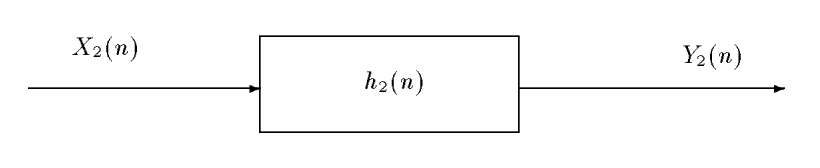
\includegraphics[width=10cm]{example.png}}
\caption{\label{fig:example} This is an example of figure included using LaTeX commands.}
\end{figure}
\end{listing}

which renders as

\begin{figure}
\centerline{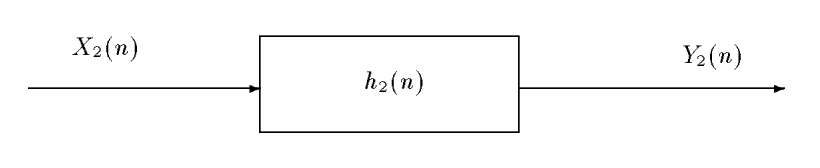
\includegraphics[width=10cm]{example.png}}
\caption{\label{fig:example} This is an example of figure included using LaTeX commands.}
\end{figure}

Of course, this Figure can now be referenced:

\begin{listing}
Figure \ref{fig:example} shows a second filter with input $X_2$, output $Y_2$  and an impulse response denoted as $h_2(n)$
\end{listing}

Figure \ref{fig:example} shows a second filter with input \(X_2\),
output \(Y_2\) and an impulse response denoted as \(h_2(n)\)

    \subsection{figcaption}\label{figcaption}

    For Python user, we have added in passing a simple function in the
\texttt{latex\_envs.py} library. This function can be imported
classicaly, eg \texttt{from\ latex\_envs\ import\ figcaption}. Then,
this function enables to specify a caption and a label for the next
plot. In turn, when exporting to \(\LaTeX\), the corresponding plot is
converted to a nice figure environement with a label and a caption.

    \begin{Verbatim}[commandchars=\\\{\}]
{\color{incolor}In [{\color{incolor}2}]:} \PY{o}{\PYZpc{}}\PY{k}{matplotlib} inline
        \PY{k+kn}{import} \PY{n+nn}{matplotlib}\PY{n+nn}{.}\PY{n+nn}{pyplot} \PY{k}{as} \PY{n+nn}{plt}
        \PY{k+kn}{from} \PY{n+nn}{jupyter\PYZus{}contrib\PYZus{}nbextensions}\PY{n+nn}{.}\PY{n+nn}{nbconvert\PYZus{}support}\PY{n+nn}{.}\PY{n+nn}{latex\PYZus{}envs} \PY{k}{import} \PY{n}{figcaption}
        \PY{k+kn}{from} \PY{n+nn}{numpy} \PY{k}{import} \PY{n}{pi}\PY{p}{,} \PY{n}{sin}\PY{p}{,} \PY{n}{arange}
        \PY{n}{figcaption}\PY{p}{(}\PY{l+s+s2}{\PYZdq{}}\PY{l+s+s2}{This is a nice sine wave}\PY{l+s+s2}{\PYZdq{}}\PY{p}{,} \PY{n}{label}\PY{o}{=}\PY{l+s+s2}{\PYZdq{}}\PY{l+s+s2}{fig:mysin}\PY{l+s+s2}{\PYZdq{}}\PY{p}{)}
        \PY{n}{plt}\PY{o}{.}\PY{n}{plot}\PY{p}{(}\PY{n}{sin}\PY{p}{(}\PY{l+m+mi}{2}\PY{o}{*}\PY{n}{pi}\PY{o}{*}\PY{l+m+mf}{0.01}\PY{o}{*}\PY{n}{arange}\PY{p}{(}\PY{l+m+mi}{100}\PY{p}{)}\PY{p}{)}\PY{p}{)}
\end{Verbatim}

    
    \begin{verbatim}
<IPython.core.display.HTML object>
    \end{verbatim}

    
            \begin{Verbatim}[commandchars=\\\{\}]
{\color{outcolor}Out[{\color{outcolor}2}]:} [<matplotlib.lines.Line2D at 0x894b5f8>]
\end{Verbatim}
        
    \begin{center}
    \adjustimage{max size={0.9\linewidth}{0.9\paperheight}}{latex_env_doc_files/latex_env_doc_27_2.png}
    \end{center}
    { \hspace*{\fill} \\}
    
    \subsection{Other features}\label{other-features}

    \begin{itemize}
\tightlist
\item
  As shown in the examples, eg \ref{example:mixing}, it is possible to
  mix LaTeX and markdown markup in environments\\
\item
  Environments can be nested. However, it is not possible, because of
  limlitations of regular expressions, to nest environments of the same
  king (eg itemize into itemize into itemize\ldots{})
\end{itemize}

    \subsection{User interface}\label{user-interface}

    \subsubsection{Buttons on main toolbar}\label{buttons-on-main-toolbar}

    On the main toolbar, the extension provides three buttons

\includegraphics{main_toolbar.png} The first one can be used to refresh
the numerotation of equations and references in all the document. The
second one fires the reading of the bibliography bibtex file and creates
(or updates) the reference section. Finally the third one is a toogle
button that opens or closes the configuration toolbar.

    \subsubsection{Configuration toolbar}\label{configuration-toolbar}

    The configuration toolbar 
\includegraphics{configuration_toolbar.png}
enables to enter some configuration options for the extension. First,
one can indicate the name of the bibtex file. If this file is not found
and the user creates the reference section, then this section will
indicate that the file was not found. The references drop-down menu
enables to choose the type of reference calls. The Equations input box
enable to initiate numbering of equations at the given number (this may
be useful for complex documents in several files/parts). Finally the
last drop-down menu let the user choose to number equation or to display
their label instead. These configuration options are then stored in the
notebook's metadata (and restored on reload).

    \section{Installation, usage and further
examples}\label{installation-usage-and-further-examples}

    \subsection{Installation}\label{installation}

    The extension consists in several javascript scripts:
\texttt{latex\_envs.js}, \texttt{thmsInNb4.js}, \texttt{bibInNb4.js} and
\texttt{initNb.js}, together with a stylesheet \texttt{latex\_envs.css}.
You may follow the instructions in the
\href{https://github.com/ipython-contrib/IPython-notebook-extensions/wiki}{wiki}
to install the extension.

Definitively, the simplest way to install and enable the extension is to
follow the instrutions in the
\href{https://github.com/ipython-contrib/Jupyter-notebook-extensions/blob/master/README.md}{Jupyter-notebook-extensions
repo}. Once this is done, you can open a tab at
\texttt{http://localhost:8888/nbextensions} to anable and configurate
the various extensions.

    \subsection{First example (continued)}\label{first-example-continued}

    We continue the first example on fthe Fourier transform definition
\ref{def:FT} in order to show that, of course, we can illustrate things
using a simple code. Since the Fourier transform is an essential tool in
signal processing, We put this in evidence using the \texttt{textboxa}
environment -- which is defined here in the css, and that one should
define in the LaTeX counterpart:

\begin{listing}
\begin{textboxa}
The Fourier transform is an extremely useful tool to have in your toolbox!
\end{textboxa}
\end{listing}

    \begin{textboxa}
The Fourier transform is an extremely useful tool to have in your toolbox!
\end{textboxa}

    The Fourier transform of a pure cosine is given by \[
X[k] = \frac{1}{2} \left( \delta[k-k_0] + \delta[k-k_0] \right), 
\] modulo \(N\). This is illustrated in the following simple script:

    \begin{Verbatim}[commandchars=\\\{\}]
{\color{incolor}In [{\color{incolor}3}]:} \PY{o}{\PYZpc{}}\PY{k}{matplotlib} inline
        \PY{k+kn}{import} \PY{n+nn}{numpy} \PY{k}{as} \PY{n+nn}{np}
        \PY{k+kn}{import} \PY{n+nn}{matplotlib}\PY{n+nn}{.}\PY{n+nn}{pyplot} \PY{k}{as} \PY{n+nn}{plt} 
        \PY{k+kn}{from} \PY{n+nn}{numpy}\PY{n+nn}{.}\PY{n+nn}{fft} \PY{k}{import} \PY{n}{fft}
        \PY{n}{k0}\PY{o}{=}\PY{l+m+mi}{4}\PY{p}{;} \PY{n}{N}\PY{o}{=}\PY{l+m+mi}{128}\PY{p}{;} \PY{n}{n}\PY{o}{=}\PY{n}{np}\PY{o}{.}\PY{n}{arange}\PY{p}{(}\PY{n}{N}\PY{p}{)}\PY{p}{;} \PY{n}{k}\PY{o}{=}\PY{n}{np}\PY{o}{.}\PY{n}{arange}\PY{p}{(}\PY{n}{N}\PY{p}{)}
        \PY{n}{x}\PY{o}{=}\PY{n}{np}\PY{o}{.}\PY{n}{sin}\PY{p}{(}\PY{l+m+mi}{2}\PY{o}{*}\PY{n}{np}\PY{o}{.}\PY{n}{pi}\PY{o}{*}\PY{n}{k0}\PY{o}{*}\PY{n}{n}\PY{o}{/}\PY{n}{N}\PY{p}{)}
        \PY{n}{X}\PY{o}{=}\PY{n}{fft}\PY{p}{(}\PY{n}{x}\PY{p}{)}
        \PY{n}{plt}\PY{o}{.}\PY{n}{stem}\PY{p}{(}\PY{n}{k}\PY{p}{,}\PY{n}{np}\PY{o}{.}\PY{n}{abs}\PY{p}{(}\PY{n}{X}\PY{p}{)}\PY{p}{)}
        \PY{n}{plt}\PY{o}{.}\PY{n}{xlim}\PY{p}{(}\PY{p}{[}\PY{l+m+mi}{0}\PY{p}{,} \PY{l+m+mi}{20}\PY{p}{]}\PY{p}{)}
        \PY{n}{plt}\PY{o}{.}\PY{n}{title}\PY{p}{(}\PY{l+s+s2}{\PYZdq{}}\PY{l+s+s2}{Fourier transform of a cosine}\PY{l+s+s2}{\PYZdq{}}\PY{p}{)}
        \PY{n}{\PYZus{}}\PY{o}{=}\PY{n}{plt}\PY{o}{.}\PY{n}{xlabel}\PY{p}{(}\PY{l+s+s2}{\PYZdq{}}\PY{l+s+s2}{Frequency index (k)}\PY{l+s+s2}{\PYZdq{}}\PY{p}{)}
\end{Verbatim}

    \begin{center}
    \adjustimage{max size={0.9\linewidth}{0.9\paperheight}}{latex_env_doc_files/latex_env_doc_42_0.png}
    \end{center}
    { \hspace*{\fill} \\}
    
    \subsection{Second example}\label{second-example}

    This example shows a series of environments, with different facets;
\textbf{links, references, markdown or/and LaTeX formatting within
environments}. The listing of environments below is typed using the
environment \emph{listing}\ldots{}

    \begin{listing}
\begin{definition} \label{def:diffeq}
We call \textbf{difference equation} an equation of the form
$$
\label{eq:diffeq}
y[n]= \sum_{k=1}^{p} a_k y[n-k] + \sum_{i=0}^q b_i x[n-i]
$$
\end{definition}

\begin{property}
If all the $a_k$ in equation (\ref{eq:diffeq}) of definition \ref{def:diffeq} are zero, then the filter has a **finite impulse response**. 
\end{property}

\begin{proof}
Let $\delta[n]$ denote the Dirac impulse. Take $x[n]=\delta[n]$ in (\ref{eq:diffeq}). This yields, by definition, the impulse response:
$$
\label{eq:fir}
h[n]= \sum_{i=0}^q b_i \delta[n-i],
$$
which has finite support. 
\end{proof}

\begin{theorem}
The poles of a causal stable filter are located within the unit circle in the complex plane.
\end{theorem}

\begin{example} \label{ex:IIR1}
Consider $y[n]= a y[n-1] +  x[n]$. The pole of the transfer function is $z=a$. The impulse response $h[n]=a^n$ has infinite support.
\end{example}

In the following exercise, you will check that the filter is stable iff $a$<1.

\begin{exercise}\label{ex:exofilter}
Consider the filter defined in Example \ref{ex:IIR1}. Using the **function** `lfilter` of scipy, compute and plot the impulse response for several values of $a$.
\end{exercise}

\end{listing}

    The lines above are rendered as follows (of course everything can be
tailored in the stylesheet):

\begin{definition} \label{def:diffeq}
We call \textbf{difference equation} an equation of the form
\begin{equation}
\label{eq:diffeq}
y[n]= \sum_{k=1}^{p} a_k y[n-k] + \sum_{i=0}^q b_i x[n-i]
\end{equation}
\end{definition}

Properties of the filter are linked to the coefficients of the
difference equation. For instance, an immediate property is

\begin{property}
If all the $a_k$ in equation (\ref{eq:diffeq}) of definition \ref{def:diffeq} are zero, then the filter has a **finite impulse response**. 
\end{property}

\begin{proof}
Let $\delta[n]$ denote the Dirac impulse. Take $x[n]=\delta[n]$ in (\ref{eq:diffeq}). This yields, by definition, the impulse response:
\begin{equation}
\label{eq:fir}
h[n]= \sum_{i=0}^q b_i \delta[n-i],
\end{equation}
which has finite support. 
\end{proof}

\begin{theorem}
The poles of a causal stable filter are located within the unit circle in the complex plane.
\end{theorem}

\begin{example} \label{ex:IIR1}
Consider $y[n]= a y[n-1] +  x[n]$. The pole of the transfer function is $z=a$. The impulse response $h[n]=a^n$ has infinite support.
\end{example}

In the following exercise, you will check that the filter is stable iff
\(a\)\textless{}1.

\begin{exercise}\label{ex:exofilter}
Consider the filter defined in Example \ref{ex:IIR1}. Using the **function** `lfilter` of scipy, compute and plot the impulse response for several values of $a$.
\end{exercise}

    \begin{listing}
The solution of exercise \ref{ex:exofilter}, which uses a difference equation as in Definition \ref{def:diffeq}:
\end{listing}

The solution of exercise \ref{ex:exofilter}, which uses a difference
equation as in Definition \ref{def:diffeq}:

    \begin{Verbatim}[commandchars=\\\{\}]
{\color{incolor}In [{\color{incolor}4}]:} \PY{o}{\PYZpc{}}\PY{k}{matplotlib} inline
        \PY{k+kn}{import} \PY{n+nn}{numpy} \PY{k}{as} \PY{n+nn}{np}
        \PY{k+kn}{import} \PY{n+nn}{matplotlib}\PY{n+nn}{.}\PY{n+nn}{pyplot} \PY{k}{as} \PY{n+nn}{plt} 
        \PY{k+kn}{from} \PY{n+nn}{scipy}\PY{n+nn}{.}\PY{n+nn}{signal} \PY{k}{import} \PY{n}{lfilter}
        \PY{n}{d}\PY{o}{=}\PY{n}{np}\PY{o}{.}\PY{n}{zeros}\PY{p}{(}\PY{l+m+mi}{100}\PY{p}{)}\PY{p}{;} \PY{n}{d}\PY{p}{[}\PY{l+m+mi}{0}\PY{p}{]}\PY{o}{=}\PY{l+m+mi}{1} \PY{c+c1}{\PYZsh{}dirac impulse}
        \PY{n}{alist}\PY{o}{=}\PY{p}{[}\PY{l+m+mf}{0.2}\PY{p}{,} \PY{l+m+mf}{0.8}\PY{p}{,} \PY{l+m+mf}{0.9}\PY{p}{,} \PY{l+m+mf}{0.95}\PY{p}{,} \PY{l+m+mf}{0.99}\PY{p}{,} \PY{l+m+mf}{0.999}\PY{p}{,} \PY{l+m+mf}{1.001}\PY{p}{,} \PY{l+m+mf}{1.01}\PY{p}{]}
        \PY{k}{for} \PY{n}{a} \PY{o+ow}{in} \PY{n}{alist}\PY{p}{:}
            \PY{n}{h}\PY{o}{=}\PY{n}{lfilter}\PY{p}{(}\PY{p}{[}\PY{l+m+mi}{1}\PY{p}{]}\PY{p}{,} \PY{p}{[}\PY{l+m+mi}{1}\PY{p}{,} \PY{o}{\PYZhy{}}\PY{n}{a}\PY{p}{]}\PY{p}{,}\PY{n}{d}\PY{p}{)}
            \PY{n}{\PYZus{}}\PY{o}{=}\PY{n}{plt}\PY{o}{.}\PY{n}{plot}\PY{p}{(}\PY{n}{h}\PY{p}{,} \PY{n}{label}\PY{o}{=}\PY{l+s+s2}{\PYZdq{}}\PY{l+s+s2}{a=}\PY{l+s+si}{\PYZob{}\PYZcb{}}\PY{l+s+s2}{\PYZdq{}}\PY{o}{.}\PY{n}{format}\PY{p}{(}\PY{n}{a}\PY{p}{)}\PY{p}{)}
        \PY{n}{plt}\PY{o}{.}\PY{n}{ylim}\PY{p}{(}\PY{p}{[}\PY{l+m+mi}{0}\PY{p}{,}\PY{l+m+mf}{1.5}\PY{p}{]}\PY{p}{)}
        \PY{n}{plt}\PY{o}{.}\PY{n}{xlabel}\PY{p}{(}\PY{l+s+s1}{\PYZsq{}}\PY{l+s+s1}{Time}\PY{l+s+s1}{\PYZsq{}}\PY{p}{)}
        \PY{n}{\PYZus{}}\PY{o}{=}\PY{n}{plt}\PY{o}{.}\PY{n}{legend}\PY{p}{(}\PY{p}{)}
\end{Verbatim}

    \begin{center}
    \adjustimage{max size={0.9\linewidth}{0.9\paperheight}}{latex_env_doc_files/latex_env_doc_48_0.png}
    \end{center}
    { \hspace*{\fill} \\}
    
    \subsection{Third example:}\label{third-example}

    This example shows that environments like itemize or enumerate are also
available. As already indicated, this is useful for copying text from a
TeX file. Following the same idea, text formating commands
\texttt{\textbackslash{}textit}, \texttt{\textbackslash{}textbf},
\texttt{\textbackslash{}underline}, etc are also available.

    \begin{listing}
The following \textit{environments} are available:
\begin{itemize}
    \item \textbf{Theorems and likes}
    \begin{enumerate}
        \item theorem,
        \item lemma,
        \item corollary
        \item ...
    \end{enumerate}
    \item \textbf{exercises}
    \begin{enumerate}
        \item problem,
        \item example,
        \item exercise
    \end{enumerate}
\end{itemize}
\end{listing}

    which gives\ldots{}

The following \textit{environments} are available:

\begin{itemize}
\item \textbf{Theorems and likes}
\begin{enumerate}
\item theorem,
\item lemma,
\item corollary
\item ...
\end{enumerate}
\item \textbf{exercises}
\begin{enumerate}
\item problem,
\item example,
\item exercise
\end{enumerate}
\end{itemize}

    \section{Conversion to LaTeX and
HTML}\label{conversion-to-latex-and-html}

    The extension works in the live-notebook. Since it relies on a bunch of
javascript, the notebook does not render as is in services such as
\texttt{nbviewer} or \texttt{github} viewer. Similarly,
\texttt{nbconvert} does not know of the LaTeX constructs which are used
here and therefore does not fully convert notebooks using this
extension.

Therefore, we provide specialized templates and exporters to achieve
these conversions.

    \subsection{Conversion to html}\label{conversion-to-html}

We provide a template \texttt{latex\_envs.tpl} and an exporter class
\texttt{LenvsHTMLExporter} (in library \texttt{latex\_envs.py}). Using
that class, conversion simply amounts to

\begin{verbatim}
jupyter nbconvert --to latex_envs.LenvsHTMLExporter FILE.ipynb
\end{verbatim}

A shortcut is also provided

\begin{verbatim}
jupyter nbconvert --to html_lenvs FILE.ipynb
\end{verbatim}

It should be noted that the rendering is done exactly in the same way as
in the livenotebook. Actually, it is the very same javascript which is
run in the html file. The javascript functions are available on the
\texttt{jupyter\_notebook\_extensions} CDN, which means that the
rendering of the html files requires an internet connection (this is
also true for the rendering of equations with MathJax).

\subsection{Conversion to LaTeX}\label{conversion-to-latex}

We provide two templates \texttt{thmsInNb\_article.tplx} and
\texttt{thmsInNb\_report.tplx} for article and report styles
respectively. Anyway one can also use the standard article, report, book
templates provided with nbconvert. Simply, we have improved some of the
internals styles. More importantly, we provide an exporter class
\texttt{LenvsLatexExporter} (also in library \texttt{latex\_envs.py}).
Using that class, conversion simply amounts to

\begin{verbatim}
jupyter nbconvert --to latex_envs.LenvsLatexExporter FILE.ipynb
\end{verbatim}

A shortcut is also provided

\begin{verbatim}
jupyter nbconvert --to latex_lenvs FILE.ipynb
\end{verbatim}

In addition, we provide several further options: -
\textbf{removeHeaders}: Remove headers and footers, (default false) -
\textbf{figcaptionProcess}: Process figcaptions, (default true) -
\textbf{tocrefRemove} Remove tocs and ref sections, + some cleaning,
(default true),

These options can be specified on the command line as, eg,

\begin{verbatim}
jupyter nbconvert --to latex_lenvs --LenvsLatexExporter.removeHeaders=True --  --LenvsLatexExporter.tocrefRemove=False FILE.ipynb
\end{verbatim}

    \begin{example}
As for an example, the present document has been converted using
    
    jupyter nbconvert --to latex_lenvs --LenvsLatexExporter.removeHeaders=True latex_env_doc.ipynb
    
Then the resulting file (without header/footer) has been included in the main file `documentation.tex`, where some LaTeX definitions of environments are done (namely listings, colors, etc) and compiled using 
    
    xelatex documentation
    
The output can be consulted [here](documentation.pdf).    
\end{example}

    \section{Disclaimer, sources and
thanks}\label{disclaimer-sources-and-thanks}

    This is done in th ehope it can be useful. However there are many
impovements possible, in the code and in the documentation.

\textbf{Contributions will be welcome and deeply appreciated.}

Originally, I used a piece of code from the nice online markdown editor
\texttt{stackedit}
\url{https://github.com/benweet/stackedit/issues/187}, where the authors
also considered the problem of incorporating LaTeX markup in their
markdown.

I also studied and used examples and code from
\url{https://github.com/ipython-contrib/IPython-notebook-extensions}.

    \section{References}\label{references}

(P'erez and Granger, 2007) P'erez Fernando and Granger Brian E.,
``\emph{IPython: a System for Interactive Scientific Computing}'',
Computing in Science and Engineering, vol.~9, number 3, pp.~21--29, May
2007. \href{http://ipython.org}{online}

(McKinney, 2012) Wes McKinney, ``\emph{Python for data analysis: Data
wrangling with Pandas, NumPy, and IPython}'', 2012.

(Rossant, 2013) Cyrille Rossant, ``\emph{Learning IPython for
interactive computing and data visualization}'', 2013.

(Shen, 2014) Shen Helen, ``\emph{Interactive notebooks: Sharing the
code}'', Nature, vol.~515, number 7525, pp.~151--152, 2014.


    % Add a bibliography block to the postdoc
    
    
    
    \end{document}
